\documentclass{beamer}
\usepackage{verbatim}
\usepackage{graphicx}
\graphicspath{ {images/} }

\title[Forum Presentation]{COSC3500 Forum Presentation}
\author{Max Bo}
\date{22nd of October}

\begin{document}

\begin{frame}
  \titlepage
\end{frame}

% The presentations will be marked out of 5 according to the following general criteria:

% General presentation technique (/1.5)

% Depth and detail; comparing commonalities (/2.5)

% Question time: demonstrating correctness of work and understanding of concepts (1)

\begin{frame}{Outline}
 \tableofcontents
\end{frame}

% \section{Introduction}

% \begin{frame}{Introduction}

% \begin{itemize}
%   \item Your introduction goes here!
% \end{itemize}

\begin{frame}{Description}
\section{Description}
The task was to create a stock-standard, 2-dimensional gravitational $n$-body simulator. 

\vskip 1cm

All bodies were to be assumed to be point masses. The simulation was to be accurate, maintaining a constant total energy, and exhibiting phenomena such as apsidal precession. 
\end{frame}

\begin{frame}{Demo}
\section{Demo}
\end{frame}

\begin{frame}[allowframebreaks]{Integration}
\section{Integration}

\[
  F = G \frac{m_1 m_2}{r^2}
\]

\begin{align*}
a_{i}&=F(x_{i})\\
v_{i+1}&=v_{i}+a_{i}\,\Delta t\\
\end{align*}

\framebreak

Dehen and Read note that the Euler method `performs very poorly in practice', further noting that `errors are proportional to $\Delta t^2$'. They contrast it with the second-order \textit{Leapfrog} symplectic integrator, which is `heavily used in collisionless N-body applications'.

\begin{align*}
x_{i}&=x_{i-1}+v_{i-1/2}\,\Delta t\\
a_{i}&=F(x_{i})\\
v_{i+1/2}&=v_{i-1/2}+a_{i}\,\Delta t\\
\end{align*}

which only requires a single acceleration calculation per every two half timesteps

\framebreak

and a `kick-drift-kick' form

\begin{align*}
v_{i+1/2}&=v_{i}+a_{i}{\frac {\Delta t}{2}}\\
x_{i+1}&=x_{i}+v_{i+1/2}\Delta t\\
v_{i+1}&=v_{i+1/2}+a_{i+1}{\frac {\Delta t}{2}}
\end{align*}

that is stable with variable timstepping, but incurs an additional acceleration calculation per every two half timesteps.
\end{frame}

\begin{frame}[allowframebreaks]{Barnes-Hut}
\section{Barnes-Hut}

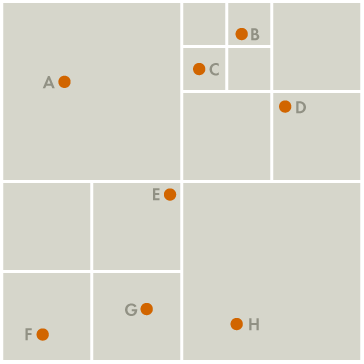
\includegraphics[width=0.6\textwidth]{quadtree}

\framebreak

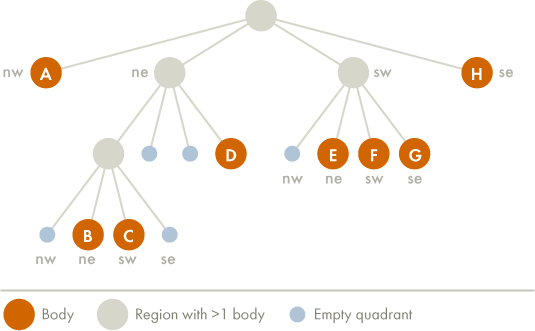
\includegraphics[width=\textwidth]{quadtree_tree}

\framebreak

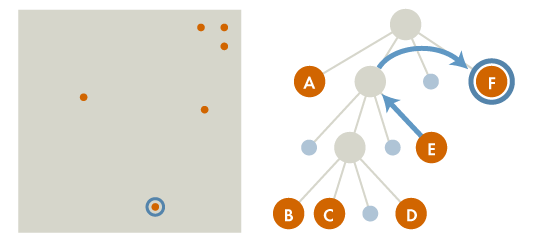
\includegraphics[width=\textwidth]{quadtree_leaf}

\framebreak

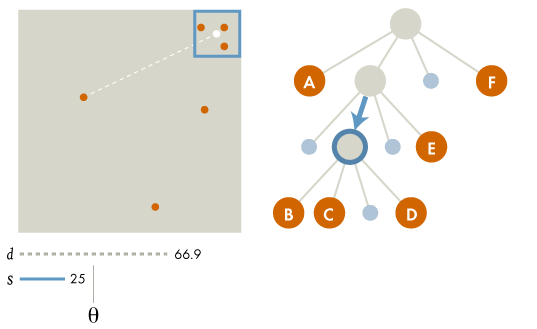
\includegraphics[width=\textwidth]{quadtree_internal}

\framebreak

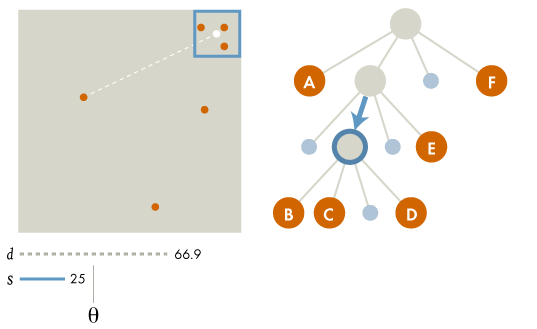
\includegraphics[width=\textwidth]{quadtree_internal}

\framebreak 

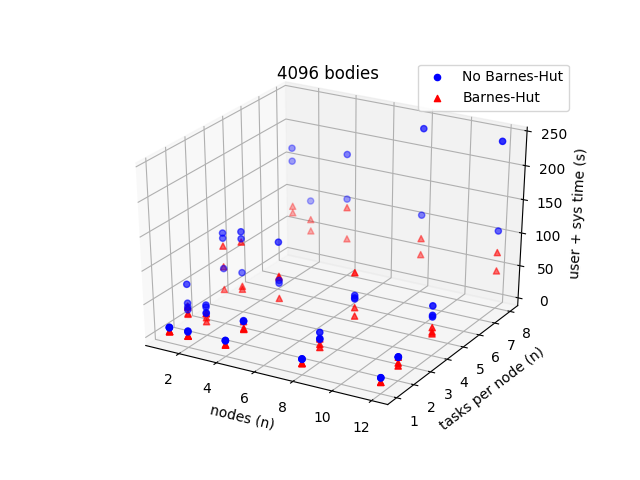
\includegraphics[width=\textwidth]{4096-nodes-tasksPerNode}

\framebreak 

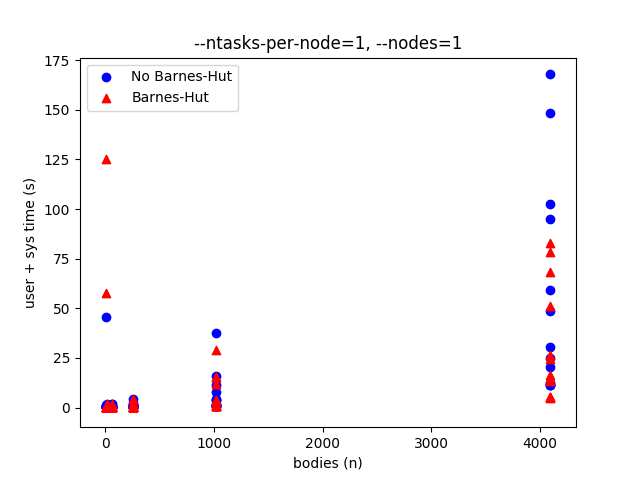
\includegraphics[width=\textwidth]{bodies_scaling}
\end{frame}

\begin{frame}[allowframebreaks]{Correctness}
\section{Correctness}
\[
U = -G\frac {mM}{R}
\]
\[
E_\text{k} =\tfrac{1}{2} mv^2 
\]

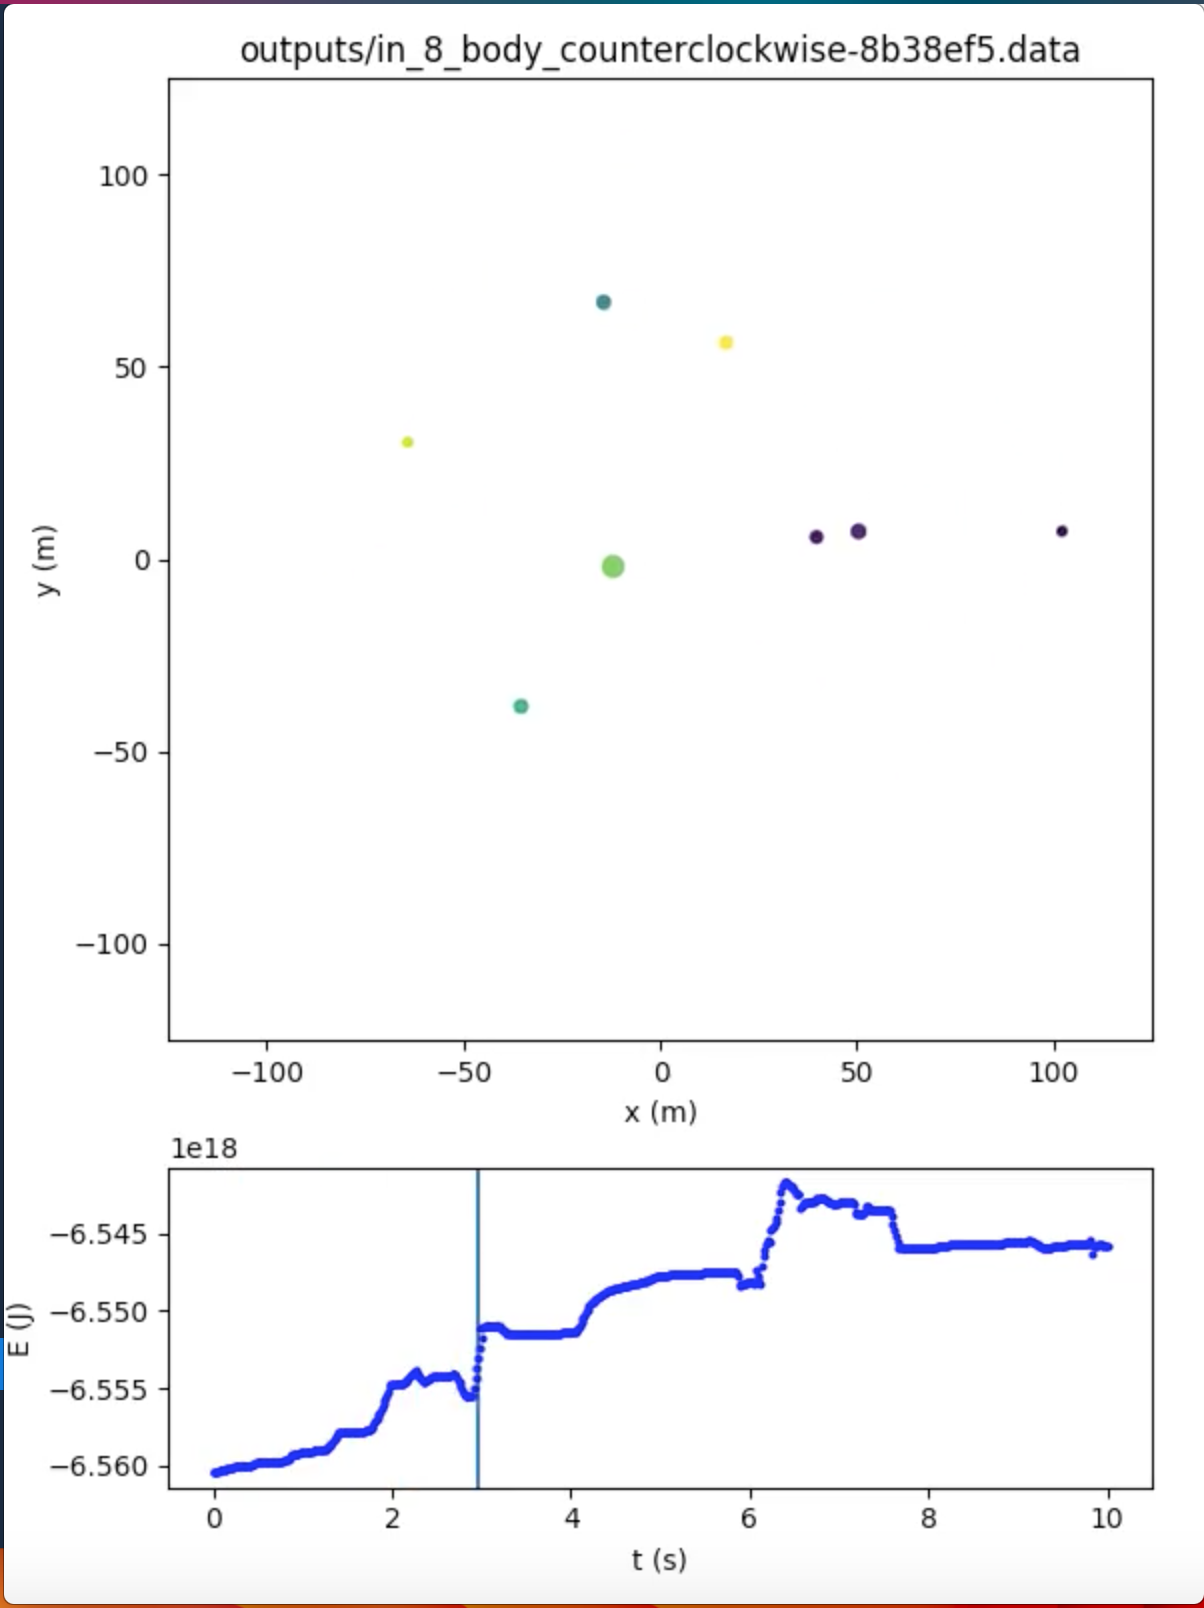
\includegraphics[width=0.5\textwidth]{barnes_hut}

\framebreak

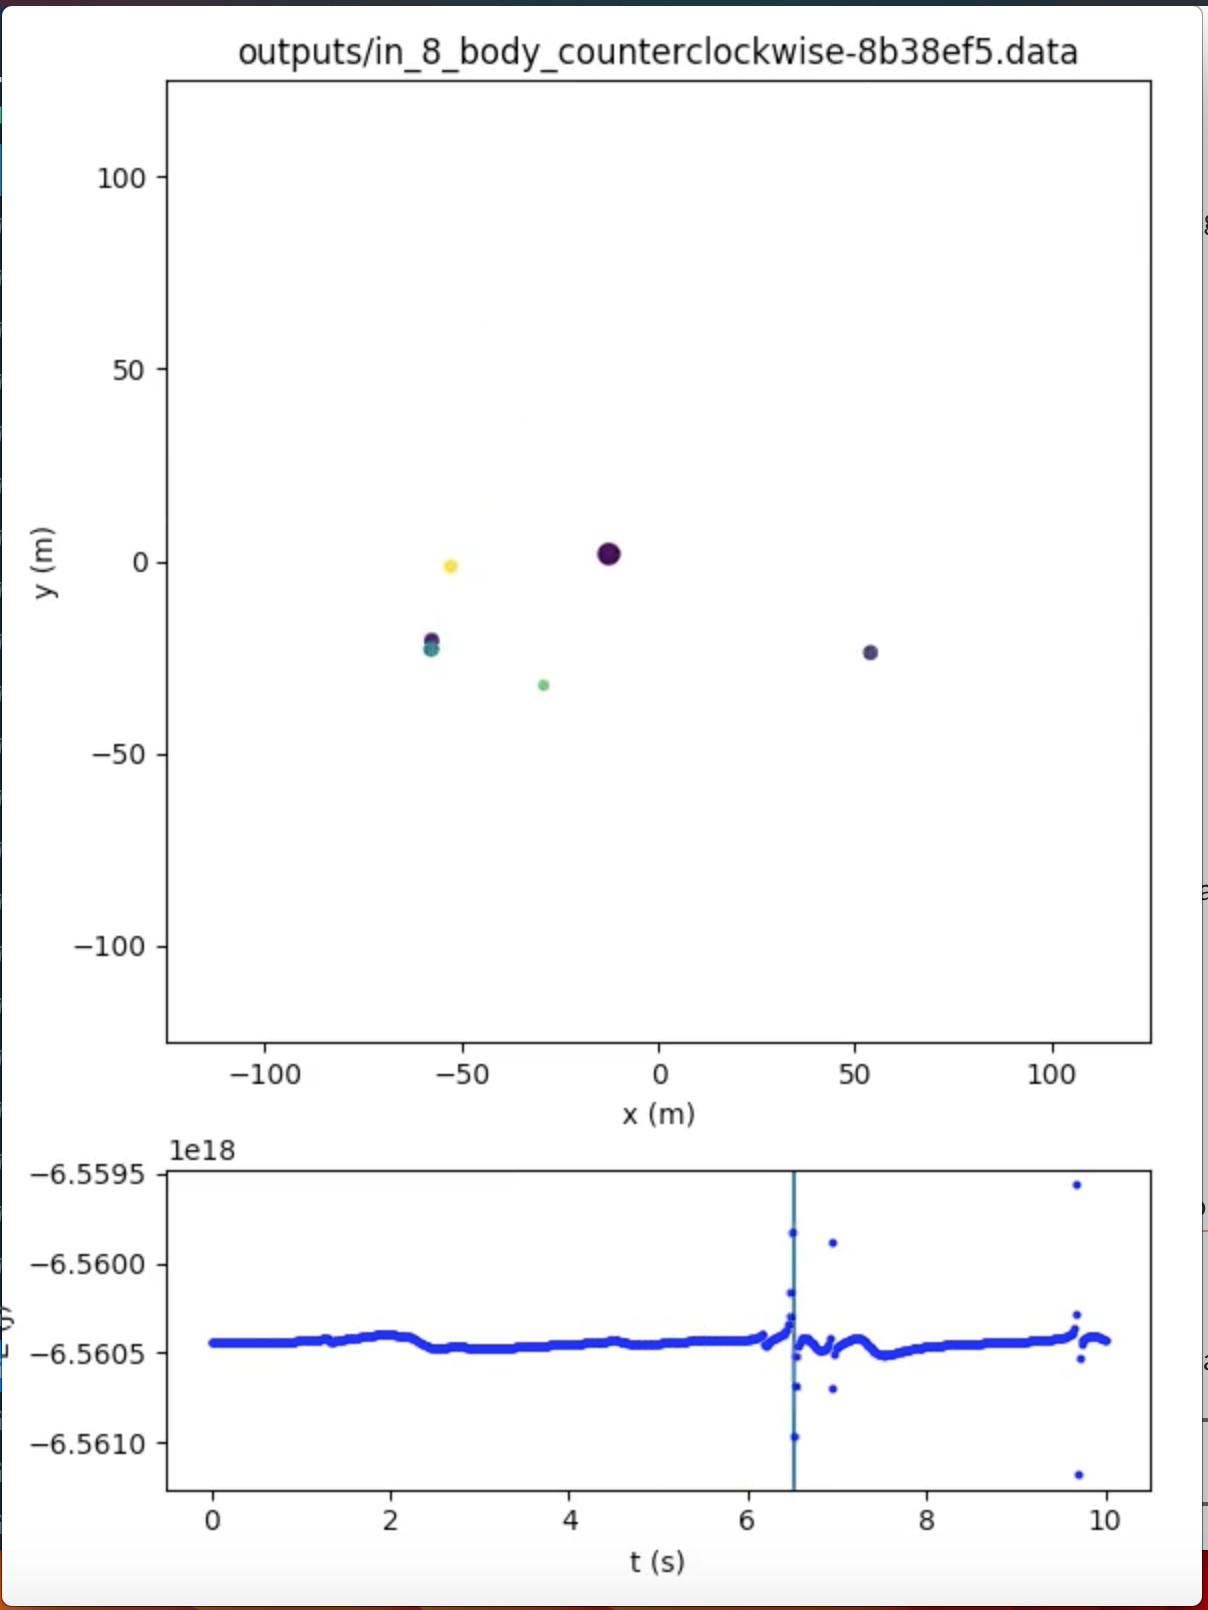
\includegraphics[width=0.5\textwidth]{energy_anomaly}
\end{frame}

\begin{frame}[allowframebreaks]{Performance Optimizations}
\section{Performance Optimizations}

\begin{align*}
a_{i}&=F(x_{i})\\
v_{i+1}&=v_{i}+a_{i}\,\Delta t
\end{align*}

\end{frame}

\begin{frame}[allowframebreaks]{Parallelization}
\section{Parallelization}

\verbatiminput{head.txt}
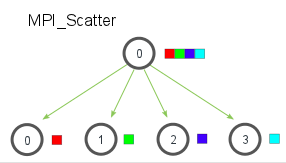
\includegraphics[width=4cm]{mpi_scatter}

\framebreak

\verbatiminput{tail.txt}

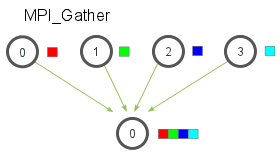
\includegraphics[width=4cm]{mpi_gather}

\framebreak

Total CPU time on rank 0 was 89.820000

Total CPU time on rank 1 was 37.040000

Total CPU time on rank 2 was 36.750000

Total CPU time on rank 3 was 36.960000

\end{frame}

\begin{frame}[allowframebreaks]{Resultss}
\section{Results}
\end{frame}

\begin{frame}[allowframebreaks]{Results}
\section{???}


\includegraphics[width=8cm]{hmm}

\framebreak

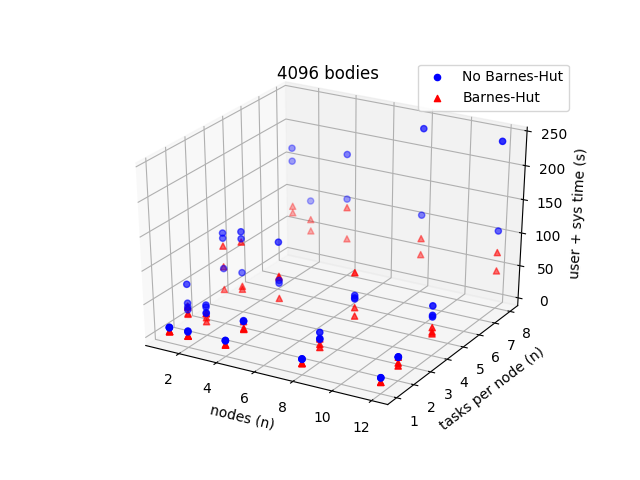
\includegraphics[width=\linewidth]{4096-nodes-tasksPerNode}

\framebreak

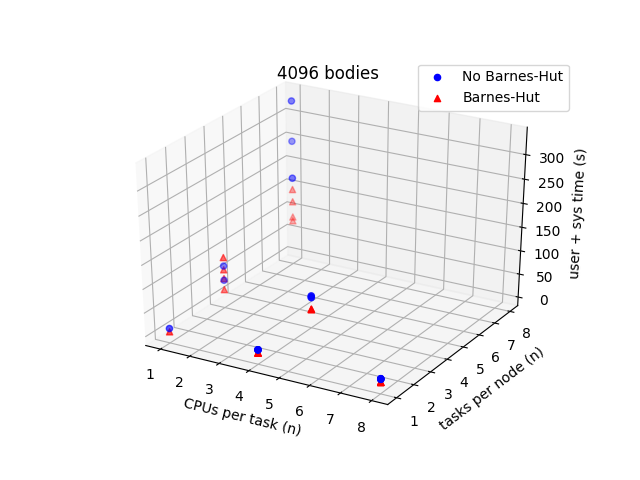
\includegraphics[width=\linewidth]{4096-cpusPerTask-tasksPerNode}

\framebreak

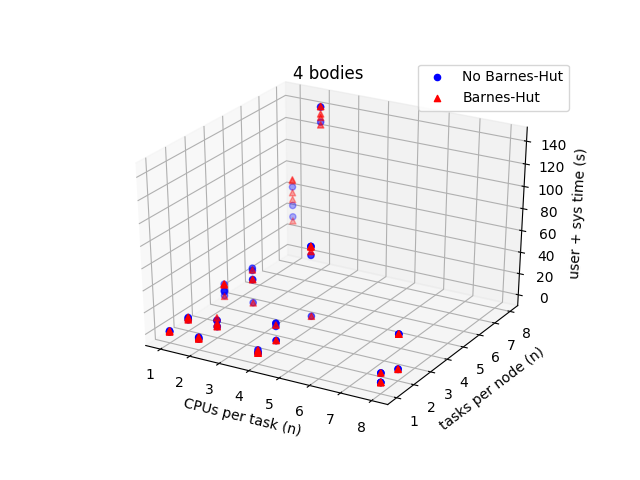
\includegraphics[width=\linewidth]{4-cpusPerTask-tasksPerNode}

\framebreak

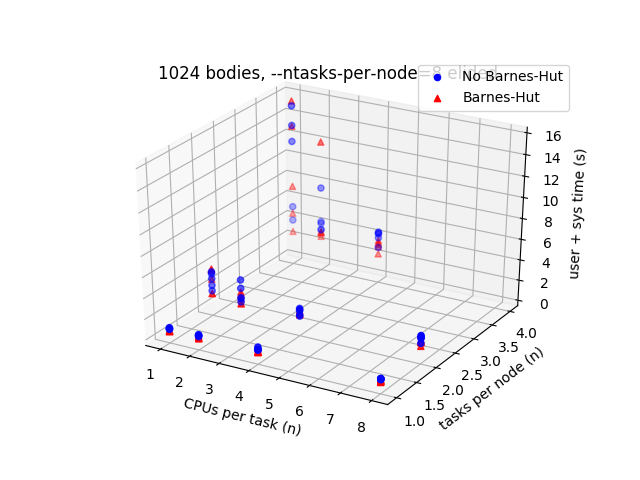
\includegraphics[width=\linewidth]{1024-cpusPerTask-tasksPerNode-elide_8_tpn}

\framebreak

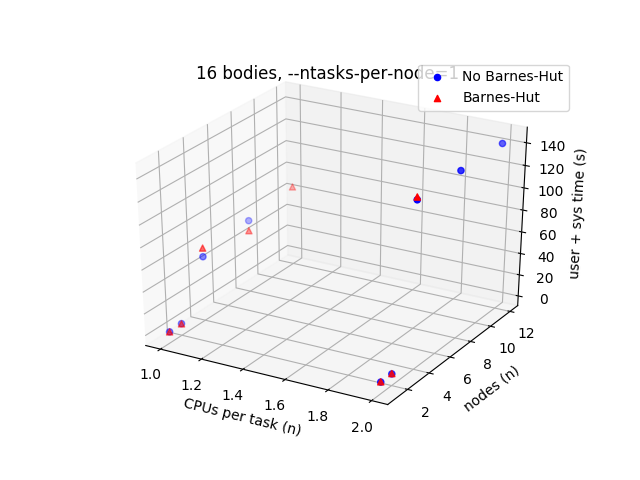
\includegraphics[width=\linewidth]{16-cpusPerTask-nodes-just_1_tpn}

\framebreak

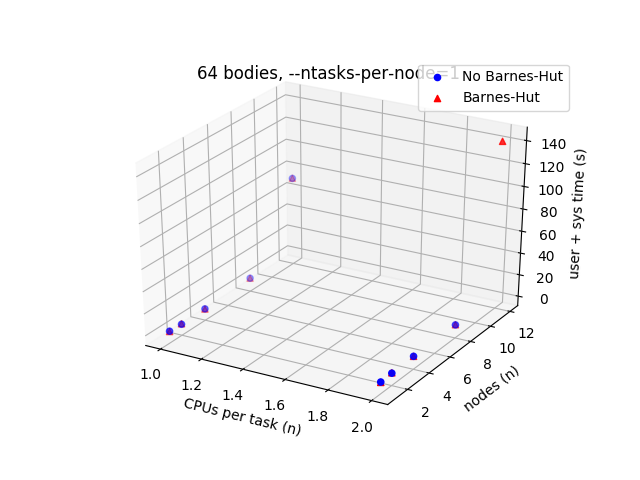
\includegraphics[width=\linewidth]{64-cpusPerTask-nodes-just_1_tpn}

\framebreak

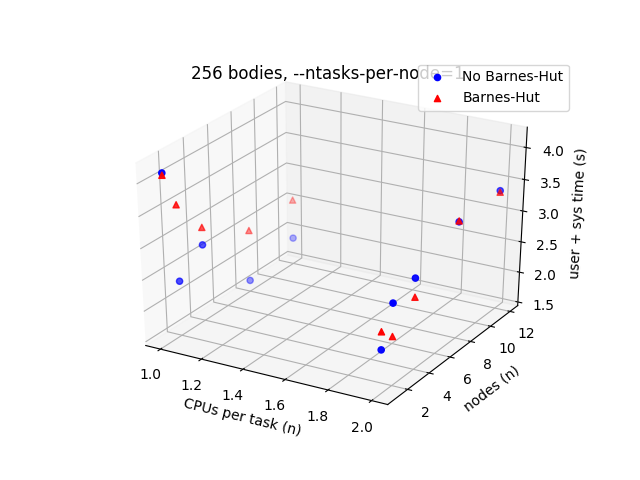
\includegraphics[width=5.2cm]{256-cpusPerTask-nodes-just_1_tpn}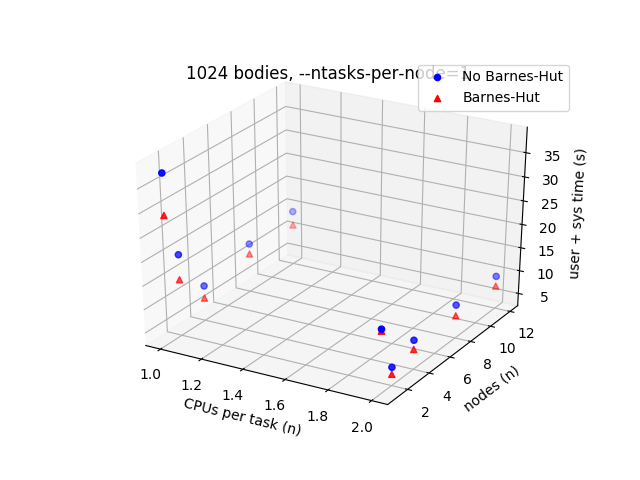
\includegraphics[width=5.2cm]{1024-cpusPerTask-nodes-just_1_tpn}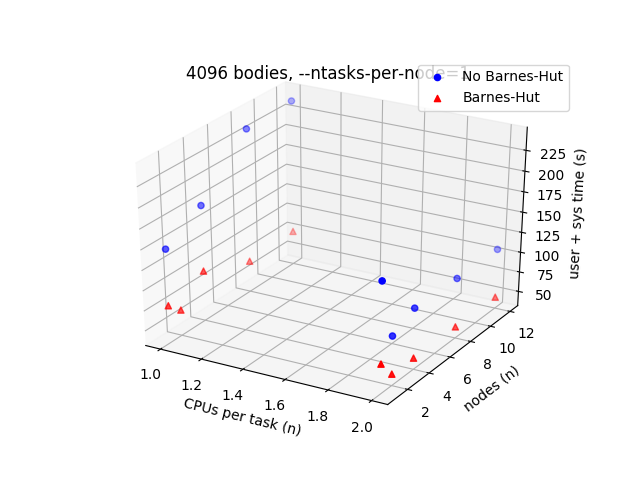
\includegraphics[width=5.2cm]{4096-cpusPerTask-nodes-just_1_tpn}

\framebreak

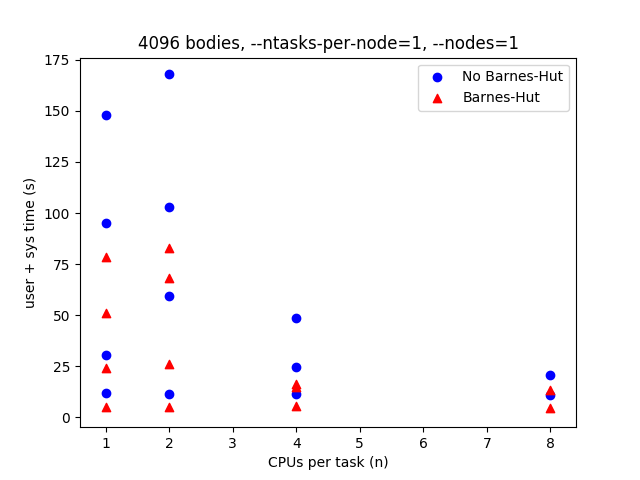
\includegraphics[width=\linewidth]{scaling}

\end{frame}

\end{document}
